\begin{figure}[t]
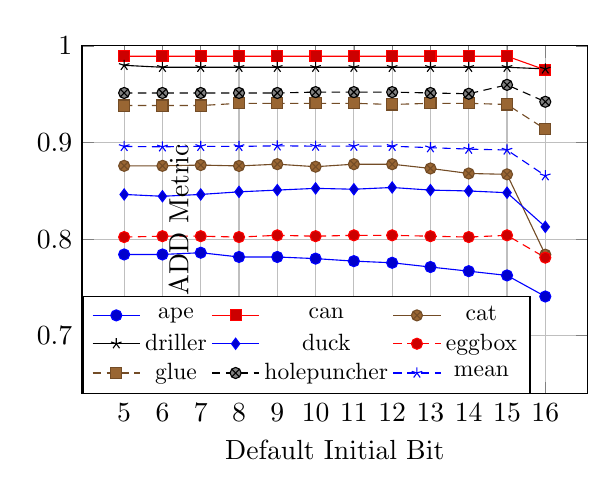
\begin{tikzpicture}
\begin{axis}[
scaled y ticks=real:100,
ytick scale label code/.code={},
ymin = 64,
ymax = 100,
symbolic x coords={5, 6, 7, 8, 9, 10, 11, 12, 13, 14, 15, 16},
xtick=data,
height=6cm,
width=8cm,
grid=major,
xlabel={Default Initial Bit},
ylabel={ADD Metric},
y label style={at={(0.23,0.5)}},
legend style={
        at={(0.445,0.0)},
        anchor=south,
        legend columns=3,
        nodes={scale=0.85, transform shape}
    },
]

\addplot coordinates {
(5,78.41) 
(6, 78.41) 
(7, 78.59) 
(8, 78.15) 
(9, 78.15) 
(10, 77.98)
(11, 77.72)
(12, 77.55)
(13, 77.11)
(14, 76.68)
(15, 76.24)
(16, 74.06)           
};


\addplot coordinates {
(5,98.92) 
(6, 98.92) 
(7, 98.92) 
(8, 98.92) 
(9, 98.92)
(10, 98.92)
(11, 98.92)
(12, 98.92)
(13, 98.92)
(14, 98.92)
(15, 98.92)
(16, 97.51)
};

\addplot coordinates {
(5,87.58) 
(6, 87.58) 
(7, 87.66) 
(8, 87.57) 
(9, 87.75)
(10, 87.49)
(11, 87.75)
(12, 87.75)
(13, 87.31)
(14, 86.79)
(15, 86.7)
(16, 78.39)
};

\addplot coordinates {
(5,97.98) 
(6, 97.78) 
(7, 97.78) 
(8, 97.78) 
(9, 97.78)
(10, 97.78)
(11, 97.78)
(12, 97.78)
(13, 97.78)
(14, 97.78)
(15, 97.78)
(16, 97.61)
};

\addplot coordinates {
(5,84.62) 
(6, 84.43) 
(7, 84.62) 
(8, 84.89) 
(9, 85.07)
(10, 85.25)
(11, 85.16)
(12, 85.34)
(13, 85.07)
(14, 84.98)
(15, 84.8)
(16, 81.27)
};

\addplot coordinates {
(5,80.21) 
(6, 80.3) 
(7, 80.3) 
(8, 80.21) 
(9, 80.39)
(10, 80.3)
(11, 80.39)
(12, 80.39)
(13, 80.3)
(14, 80.21)
(15, 80.39)
(16, 78.08)
};

\addplot coordinates {
(5,93.82) 
(6, 93.82) 
(7, 93.82) 
(8, 94.05) 
(9, 94.05)
(10, 94.05)
(11, 94.05)
(12, 93.93)
(13, 94.05)
(14, 94.05)
(15, 93.93)
(16, 91.37)
};

\addplot coordinates {
(5,95.12) 
(6, 95.12) 
(7, 95.12) 
(8, 95.12) 
(9, 95.12)
(10, 95.21)
(11, 95.21)
(12, 95.21)
(13, 95.12)
(14, 95.04)
(15, 95.96)
(16, 94.21)
};

\addplot coordinates {
(5,89.59) 
(6, 89.55) 
(7, 89.60) 
(8, 89.59) 
(9, 89.65)
(10, 89.62)
(11, 89.62)
(12, 89.61)
(13, 89.46)
(14, 89.31)
(15, 89.22)
(16, 86.56)
};

\legend{ape, can, cat, driller, duck, eggbox, glue, holepuncher, mean}
\end{axis}
\end{tikzpicture}
\vspace{-0.3cm}
     \caption{We conduct an ablation study on selecting the default initial bit $m_{default}$ using $8$ objects from the LM-O dataset.
     The flat curve illustrates that our proposed design is robust and has a clear advantage to the non-hierarchical variant ($16$ as initial bit). }
     \label{fig:ablation_initial_bit}
\end{figure}